\documentclass[main.tex]{subfiles}
\begin{document}
	
	The method presented in this \paper{} performs static code analysis on Haskell modules to determine which extensions are needed in the module, and which ones are not. For this, the algorithm needs an abstract representation of the source code. This representation is called the \emph{abstract syntax tree}, shortly referred to as \emph{AST}. The syntax tree can be constructed by an external tool, such as \cite{haskell-src-exts} or by the compiler itself. The algorithm presented here uses a syntax tree produced by a combination of these two techniques. It uses the unique representation of Haskell-Tools, which is a transformed version of the GHC syntax tree. In Diagram~\ref{fig:haskell-tools-architecture}\footnote{The diagram is taken from the Haskell-Tools \href{https://github.com/haskell-tools/haskell-tools/blob/master/documentation/haskell_tools_architecture.png}{documentation}. April 29, 2018 } we can see the outline of Haskell-Tools' architecture. In this chapter, we will discuss the various properties of the Haskell-Tools AST and present a general overview of its construction. Most of the work described in the following sections was not implemented as part of this \paper{}. 
	
	\begin{figure}[H]
		\renewcommand{\figurename}{Diagram}
		\hspace{-1cm}
		\centering
		\caption{Architecture of Haskell-Tools}
		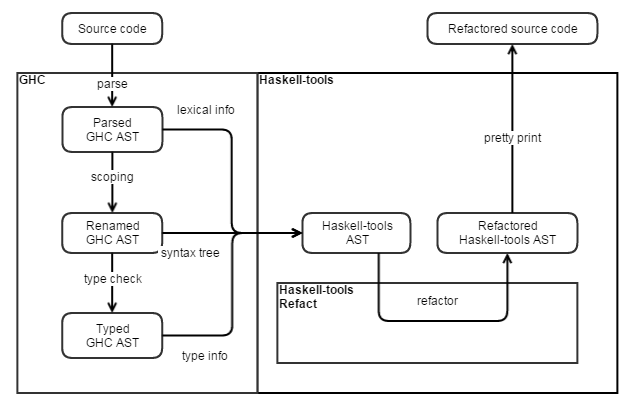
\includegraphics[scale=0.5]{haskell_tools_architecture}
		\label{fig:haskell-tools-architecture}
	\end{figure}
	
	\newpage
	
	\section{Components of Haskell-Tools}
	
	First we must examine the two main components of Haskell-Tools to understand how the extension eliminating refactoring fits into the entire infrastructure. These two components are the refactoring framework and the daemon.
	
	\subsection{Refactoring framework}
	
	The refactoring framework is responsible for providing a comprehensive refactoring infrastructure for programmers to define and integrate their own code transformations into Haskell-Tools. It consists of five sperate packages: \pilcode{ast}, \pilcode{backend-ghc}, \pilcode{pretty-print}, \pilcode{rewrite} and \pilcode{refactor}. Their dependency graph can be seen in Figure~\ref{fig:refactor-package-diagram}.
	
	Each package serves a different purpose. The \pilcode{ast} package is responsible for providing the Haskell-Tools representation of the abstract syntax tree. This representation is very well optimized for code transformations. It also defines how the syntax tree should be annotated with both semantic (type info) and source related information (comments). This package is used by nearly all other Haskell-Tools packages. 
	
	Package \pilcode{backend-ghc} is used to transform the GHC syntax tree into the internal representation. The transformation is done by extracting different versions of the AST from GHC at various stages of the compilation, and collecting the necessary information from them. Note that the representation of the syntax tree can drastically differ at each stage of the compilation. Besides transforming the AST, this package also annotates it with different kinds of semantic information such types of certain nodes.
	
	After a code transformation, we need to print the syntax tree into Haskell source code. The \pilcode{pretty-print} package does exactly that. The package is also responsible for adding source related information to the syntax tree, such as indentation, relative position of language elements and comments. Using this extra information, we can reproduce the exact same source code we constructed the AST from.
	
	A refactoring needs to do two things: finding certain nodes in the AST and transforming them. These two features are provided by the \pilcode{rewrite} package. It defines user-friendly pattern synonyms to make finding the nodes easier, and it also provides generating functions to create new syntax tree nodes from scratch. It is worth mentioning that these newly created nodes do not contain any semantic information. This means, the AST has to be reconstructed after every single refactoring.
	
	Finally, the \pilcode{refactor} package is responsible for organizing all the features presented above, and providing an easy-to-use interface for defining refactorings. It loads the modules, executes the given refactorings and supplies utility functions.
	
	Haskell-Tools also provides built-in refactorings. One of them is the extension elimination refactoring. These predefined code transformations can be found in the \pilcode{builtin-refactorings} package. This package uses all previously defined packages, this is what the big headed arrow ought to represent. Most of the work presented in this \paper{} was implemented in \pilcode{builtin-refactorings} package, but code modifications were issued to other packages as well, and some utility modules were defined too.
	
	\subfile{refactor_component}
	
	\subsection{Daemon} 
	
	The \pilcode{daemon} package is responsible for providing a main server loop for clients of Haskell-Tools. We can see its dependencies, and the processes it communicates with in Figure~\ref{fig:daemon-package-diagram}. Any given process can perform refactorings by communicating with the server using a predefined protocol. The \pilcode{daemon} also manages the resources needed to perform a refactoring, so for example it is responsible for identifying and loading the projects into memory. It is dependent on some of the packages mentioned earlier. It needs \pilcode{pretty-print} to produce human-readable log files, it also depends on \pilcode{builtin-refactorings} to access the predefined refactorings, and finally it requires \pilcode{refactor} for loading individual modules. It can establish a two-way communication with any process that implements its predefined protocol.
	
	\subfile{daemon_component}
	
	Currently, there are two client processes that implement this protocol: the command line interface and the atom integration package. \pilcode{ht-atom} is written in coffee script and is entirely independent of the \pilcode{daemon}, it only needs to know the protocol. It provides an easy-to-use graphical interface for the user to perform refactorings. Package \pilcode{cli} on the other hand is implemented in Haskell, and it does not communicate with the \pilcode{daemon}, instead calls its functions explicitly from code. This obviously has some advantages and some drawbacks as well. Its main advantage is that the entire "communication" can be handled in the type safe environment of Haskell. This minimizes the possible communication errors. However, it needs to depend on the packages indicated on Figure~\ref{fig:daemon-package-diagram}, so it has to be rebuilt every single time we modify any of these packages. Fortunately though, the \pilcode{cli} package is really small in size, so it can be compiled pretty quickly.
		
	\section{Properties of the abstract syntax tree}
	
	Despite its name, the syntax tree can contain much more information about the source code than only its syntactic structure. The individual extension checkers use two special properties of the syntax tree provided by Haskell-Tools: the semantic information carried by its nodes and also its concrete representation of the source code's syntax.
	
	\subsection{Semantic information}
	
	% semantic X vs semantical X:
	% Ask the question the: does X have meaning? If YES -> semantical, if NO -> semantical
	% semantic object, semantical ambiguity
	
	In most cases, eliminating a certain extension requires more than a syntactic analysis of the source code. From the perspective of the algorithm, the most relevant piece is the semantic information stored in the AST's nodes. There are two kinds of semantic information in the syntax tree that are particularly important: type information and unique names. As discussed in Section~\ref{ghc-exts}, some extensions can enrich the type system of GHC by new features. The type information present in certain nodes of the AST are used to determine the necessity of these extensions.
	
	In the syntax tree, not all nodes have type information associated with them. The reason for this is that the type checker discards intermediate result types after calculating them. As a result, the type information of subexpressions are lost after the type checking phase ends. As a consequence, GHC does not store type information for subexpressions, only for named program elements. In particular, only overloaded literals have directly accessible type information. Luckily, we can obtain the types of other nodes as well by using their unique names. GHC provides certain lookup functions which can recover the type of a given node based on its unique name. Haskell-Tools stores these unique names in the corresponding AST nodes. Unfortunately, using this approach, we can only access the type information of syntax tree nodes with qualified names. For instance, in the example below we can only determine the types of the function \ilcode{f}, the operator \ilcode{(:)} and the variables \ilcode{x} and \ilcode{xs}. We have no information about the subexpressions such as \ilcode{f x}.
	
	\begin{oneLineHaskell}
		map f (x:xs) = f x : map f xs
	\end{oneLineHaskell}
	
	Due to partially available type information, the individual extension checkers can only approximate the necessities of their corresponding language extensions. The algorithm presented in Section~\ref{algorithm} overcomes this issue by introducing so-called \emph{extension formulas} and \emph{certainty levels}. Using these two new constructs, despite the incomplete type information, we can eliminate most unused extensions from Haskell modules, and highlight the language elements requiring the remaining extensions.
	
	\subsection{Concrete syntax}
	
	In addition to the semantically important abstract syntax, the AST of Haskell-Tools also represents the concrete syntax of the source code. One of the main advantages of this approach, is that all the syntactic sugar present in the source code is also present in the AST. This makes the requirement checking of syntactic extensions particularly simple. Since syntactic extensions mostly only introduce some sort of syntactic sugar to the language, we only need to check the presence of the nodes corresponding to the syntactic sugar in the AST.
	
	\section{Constructing the syntax tree}
	
	The abstract syntax tree of Haskell-Tools is constructed from the AST provided by GHC. The transformation process has many different steps from which a few will be briefly outlined in this section.
	
	\subsection{Transforming the GHC representation}
	
	Haskell-Tools aims at optimizing the AST for source code transformation. One of the key steps to achieve this, is collecting all refactoring related information present in the different versions of GHC syntax trees scattered throughout the various stages of compilation. This process is required because in different stages of the compilation GHC stores different kinds of information about the AST. In some cases, between two stages certain information is lost. For example, after the renaming phase, the Template Haskell program elements are no longer present, because they are evaluated.
	
	At a certain point, the semantic information also has to be collected. This phase takes place right after all syntactic parts of the Haskell-Tools AST are constructed. For this transformation Haskell-Tools uses the type checked syntax tree of GHC. It extracts all required information from the GHC representation, and annotates its own AST with it. After the transformation, all nodes in the Haskell-Tools syntax tree will have their corresponding semantic information associated with them. It is also worth mentioning, that not all nodes have semantic information, and different types of nodes may have different types of semantic information. For instance, an operator has its fixity and its qualified name, but a literal has only its type available as semantic information.
	
	
	\subsection{Source related information}
	
	Besides storing the concrete syntactical representation of the source code, Haskell-Tools also keeps track of every bit of source related information present in the program. As a result, the original source code can be obtained from the syntax tree itself. This process is called \emph{pretty printing}. This is a really useful feature, because after performing a refactoring, we can easily generate the source code by pretty printing the syntax tree.
	
	To achieve this kind of behavior, the syntax tree has to go through several stages of transformations where the exact source ranges are calculated for the language elements, and then these ranges are replaced by the corresponding parts of the source code.
	
\end{document}